\begin{figure}
    \centering
    \begin{tikzpicture}[scale=0.75]
    \matrix[square matrix]
    {
       a&a&a&a&~&b&b&b&b&b&~&~ \\
       a&a&a&|[fill=black]|&~&b&b&b&b&b&~&~ \\
       a&a&\bf A&|[fill=black]|&~&b&b&\bf B&b&b&~&~ \\
       a&a&a&|[fill=black]|&~&b&b&b&    |[fill=black]|&|[fill=black]|&~&~ \\
       a&a&a&a&~&b&b&b&
       |[fill=black]|&~&~&~ \\
       ~&~&~&~&~&c&c&c&
       |[fill=black]|&~&~&~ \\
       ~&~&~&~&~&c&c&c&
       |[fill=black]|&~&~&~ \\
       ~&~&|[fill=black]|&~&~&c&c&\bf C&
       |[fill=black]|&~&~&~ \\
       ~&~&~&~&~&c&c&c&
       |[fill=black]|&~&~&~ \\
    };
  % \matrix[square matrix]
  %{
  %   a&a&a&a&|[fill=lightgray]|\bf \color{red}D&b&b&b&b&b&|[fill=lightgray]|\bf \color{red}E&|[fill=lightgray]|\color{red}e \\
  %   a&a&a&|[fill=black]|&|[fill=lightgray]|\color{red}d&b&b&b&b&b&|[fill=lightgray]|\color{red}e&|[fill=lightgray]|\color{red}e \\
  %   a&a&\bf A&|[fill=black]|&|[fill=lightgray]|\color{red}d&b&b&\bf B&b&b&|[fill=lightgray]|\color{red}e&|[fill=lightgray]|\color{red}e \\
  %   a&a&a&|[fill=black]|&|[fill=lightgray]|\color{red}d&b&b&b&    |[fill=black]|&|[fill=black]|&|[fill=lightgray]|\color{red}e&|[fill=lightgray]|\bf \color{red}F \\
  %   a&a&a&a&|[fill=lightgray]|\bf \color{red}G&b&b&b&
  %   |[fill=black]|&|[fill=lightgray]|\color{red}f&|[fill=lightgray]|\color{red}f&|[fill=lightgray]|\color{red}f \\
  %   |[fill=lightgray]|\bf \color{red} H&|[fill=lightgray]|\color{red}h&|[fill=lightgray]|\color{red}h&|[fill=lightgray]|\color{red}g&|[fill=lightgray]|\color{red}g&c&c&c&
  %   |[fill=black]|&|[fill=lightgray]|\color{red}f&|[fill=lightgray]|\color{red}f&|[fill=lightgray]|\color{red}f \\
  %   |[fill=lightgray]|\color{red}h&|[fill=lightgray]|\color{red}h&|[fill=lightgray]|\color{red}h&|[fill=lightgray]|\color{red}g&|[fill=lightgray]|\color{red}g&c&c&c&
  %   |[fill=black]|&|[fill=lightgray]|\bf \color{red}J&|[fill=lightgray]|\color{red}j&|[fill=lightgray]|\color{red}j \\
  %    |[fill=lightgray]|\color{red}h&|[fill=lightgray]|\color{red}h&|[fill=black]|&|[fill=lightgray]|\bf \color{red}I&|[fill=lightgray]|\color{red}i&c&c&\bf C&
  %   |[fill=black]|&|[fill=lightgray]|\color{red}j&|[fill=lightgray]|\color{red}j&|[fill=lightgray]|\color{red}j \\
  %   |[fill=lightgray]|\color{red}h&|[fill=lightgray]|\color{red}i&|[fill=lightgray]|\color{red}i&|[fill=lightgray]|\color{red}i&|[fill=lightgray]|\color{red}i&c&c&c&
  %   |[fill=black]|&|[fill=lightgray]|\color{red}j&|[fill=lightgray]|\color{red}j&|[fill=lightgray]|\color{red}j \\
  %};
    \end{tikzpicture}
    \caption{Initial centroids, and centroid marking for a grid map with $\delta = 3$.
    \textbf{A}, \textbf{B} and \textbf{C} are the obstacle-free centres of a $5 \times 5$ 
    square tiling. Cells assigned to each are marked as a, b or c.}
    \label{fig:ci}
\end{figure}


\section{Bounded Path Finding using Centroids}
\label{sec:bounded}

For some application settings, or for some types of gridmaps, it is possible 
that the space and time required to build a CPD are considered too large. 
To address such situations, we propose to compute and compress first-move 
data for only a subset of grid nodes $C$, called \emph{centroids}.

We will associate a nearest centroid $\centroid(t) \in C$ for every grid node $t$.
Then, to find a path from any $s$ to any $t$, we propose to build a
\emph{centroid path}:
$$
cp(s,t) = cpd(s,\centroid(t)) \pp \reverse(cpd(t,\centroid(t)).
$$

We can do better by joining the two paths at the first common point $p$,
which may not be $\centroid(t)$. 
$$
\begin{array}{rcl}
cp(s,t) & =  & [ n \,|\, n \in cpd(s,\centroid(t)), n \not\in cpd(t,\centroid(t))] \\
&&  \pp [ p ] \\
&& \pp [ n \,|\, n \in \reverse(cpd(t,\centroid(t)), n \not\in cpd(s,\centroid(t))] \\
p & = & \mbox{first node in $cpd(s,\centroid(t))$ also in $cpd(t,\centroid(t))$} 
\end{array}
$$

Given we have chosen centroids so that no target $t$ is more than $\delta$ from its centroid $\centroid(t)$, we can show that the 
centroid path is never longer than $2\delta$ than the optimal path.

\begin{theorem}\label{thm:centroid}
If $len(sp(t,\centroid(t)) \leq \delta$ for all $t$ in $V$, then 
$len(cp(s,t)) \leq len(sp(s,t)) + 2\delta$
\end{theorem}
\begin{proof}
Suppose for the purpose of a contradiction that we have 
\mbox{$len(cp(s,t)) > len(sp(s,t)) + 2\delta$}.
By definition, the CPD returns a path $cpd(s,\centroid(t))$ which is
a shortest possible path, and similarly for $cpd(t,\centroid(t))$, hence
we have \mbox{$len(sp(s,\centroid(t)) + len(sp(t,\centroid(t)) \geq len(cp(s,t))$}.
Consider the path $sp(s,t) \pp{} sp(t,\centroid(t))$
from $s$ to $\centroid(t)$.
By assumption, its length is at most $len(sp(s,t)) + \delta$, and hence we have that
\mbox{$len(sp(s,t)) + \delta \geq len(sp(s,\centroid(t)))$}.
Finally, we also have that \mbox{$\delta \geq len(sp(t,\centroid(t))$}.
This leads to the reasoning
$$
\begin{array}{cl}
  & len(sp(s,\centroid(t)) + len(sp(t,\centroid(t)) \\
\geq & len(cp(s,t))  \\
> & len(sp(s,t)) + 2\delta  \\
\geq & len(sp(s,\centroid(t))) + \delta \\
\geq & len(sp(s,\centroid(t))) + len(sp(t,\centroid(t)) 
\end{array}
$$
Contradiction.
\end{proof}

\begin{figure*}[t]
\begin{minipage}{0.48\textwidth}
    \centering
    \begin{tikzpicture}[scale=0.75]
   \matrix[square matrix]
   {
      a&a&a&a&\bf D&b&b&b&b&b&\bf E&e \\
      a&a&a&|[fill=black]|&d&b&b&b&b&b&e&e \\
      a&a&\bf A&|[fill=black]|&d&b&b&\bf B&b&b&e&e \\
      a&a&a&|[fill=black]|&d&b&b&b&    |[fill=black]|&|[fill=black]|&e&\bf F \\
      a&a&a&a&\bf G&b&b&b&
      |[fill=black]|&f&f&f \\
      \bf H&h&h&g&g&c&c&c&
      |[fill=black]|&f&f&f \\
      h&h&h&g&g&c&c&c&
      |[fill=black]|&\bf \bf J&j&j \\
      h&h&|[fill=black]|&\bf I&i&c&c&\bf C&
      |[fill=black]|&j&j&j \\
      h&i&i&i&i&c&c&c&
      |[fill=black]|&j&j&j \\
   };
    \end{tikzpicture}
    \caption{\small Final centroid marking after greedily adding the new centroids 
    {\bf D, E, F, G, H, I, J}, and the complete mapping of each cell to its 
    centroid.}
    \label{fig:cf}
\end{minipage}
\hspace{1em}
\begin{minipage}{0.48\textwidth}
%\begin{figure}
    \centering
    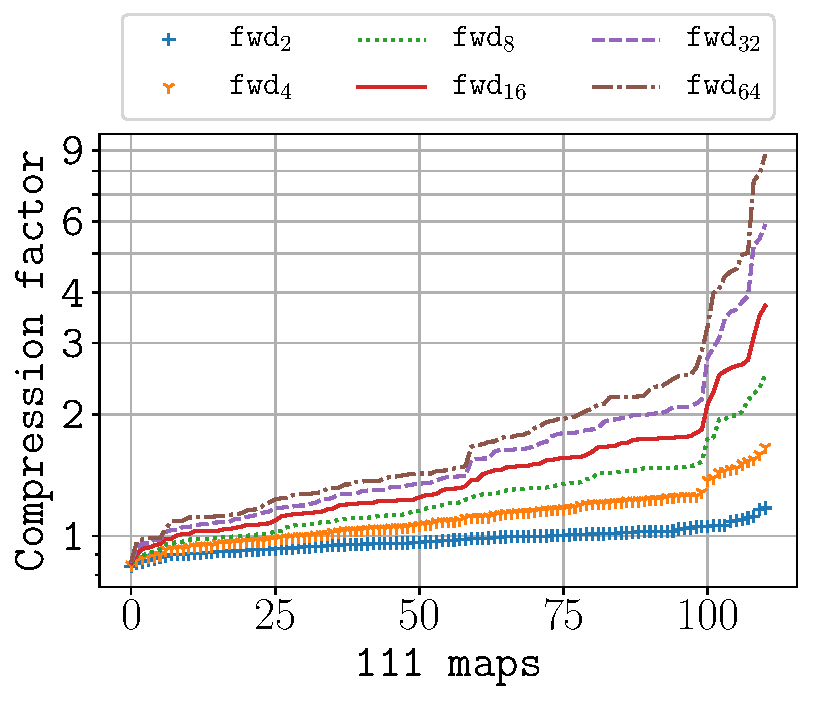
\includegraphics[width=0.9\textwidth]{pic/fwd0-fwd.pdf}
    \caption{
    \small
    Storage costs for
    suboptimal CPDs \mbox{($\delta = 2, 4, 8, 16, 32, 64$)} vs.\ optimal 
    CPDs. We test 111 maps from GPPC 2014, and report relative sizes;
    $>$ 1 is an improvement.}
    \label{fig:fwd0-fwdc}
%\end{figure}

\end{minipage}
\end{figure*}

\section{Building Centroids}
\label{sec:centroid}

The question of how to choose appropriate centroids given a radius $\delta$ is an interesting one.
In this work we propose the following simple idea.
Given $\delta$, we let $d = 1 + 2 \lfloor\frac{\delta}{\sqrt{2}} \rfloor$ be the largest value so that everything in a $d \times d$ square is within $\delta$ of the centre of the square, assuming no obstacles. 

We tile the map with non-overlapping $d \times d$ squares choosing as
(initial) centroids $C$ the centre points of these squares, if they are not
blocked or off the map.  For square $S$ with an unblocked centre $c$, we examine each cell
$t$ in the square and, if $sp(t,c) \leq \delta$, we set $\centroid(t) = c$.
Figure~\ref{fig:ci} shows an example for $\delta = 3$.


    
After the initial marking phase, we may have cells $t$ without a defined
centroid $\centroid(t)$.  For each such cell $t$, we first check if there
exists $c \in C$ s.t.\ $sp(t,c) \leq \delta$, and if so we set $\centroid(t)
= c$.  If there are multiple, we choose the closest.
Otherwise, we add $t$ to $C$ and set $c(t) = t$.  This continues until
all cells have a defined centroid.  Figure~\ref{fig:cf} shows the final 
result using the algorithm just described.



\ignore{
In practice the approach is 
somewhat cleverer, it looks for a group $G$ of connected cells
that do not have a centroid, and then chooses a new centroid from among then that is within $\delta$ of the maximum number of members of the group.  We also remap the centroids for cells $t$ with an existing centroid, if we place a new centroid closer to them.

Figure~\ref{fig:cb} shows the result of the not so greedy approach to centroid completion.

\pjs{Shizhe: check this is about right
\sz{We are using square wildcard for forward CPD, but not for reverse CPD. }

}


\begin{figure}
    \centering
    \begin{tikzpicture}
   \matrix[square matrix]
   {
      a&a&a&a&d&b&b&b&b&\color{red}e&e&e \\
      a&a&a&|[fill=black]|&d&b&b&b&b&\color{red}e&e&e \\
      a&a&\bf A&|[fill=black]|&d&\color{red}d&b&\bf B&b&\color{red}e&\bf E&e \\
      a&a&a&|[fill=black]|&\bf D&\color{red}d&b&b&    |[fill=black]|&|[fill=black]|&e&e \\
      a&a&a&\color{red}d&d&\color{red}d&b&b&
      |[fill=black]|&e&e&e \\
      f&f&f&f&d&c&c&c&
      |[fill=black]|&g&g&g \\
      f&f&\bf F&f&f&c&c&c&
      |[fill=black]|&g&g&g \\
      f&f&|[fill=black]|&f&f&c&c&\bf C&
      |[fill=black]|&g&\bf G&g \\
      h&h&\bf H&h&h&c&c&c&
      |[fill=black]|&g&g&g \\
   };
    \end{tikzpicture}
    \caption{\small Final centroids (capital letters) and centroid mapping for a grid map, using clever addition of new centroids, and remapping cells (in red) to their closest centroid.}
    \label{fig:cb}
    \end{figure}

\pjs{Do we need a figure of number of cells/number of centroids for the maps to show the "expected compression ratio"}

}

With the marking complete, we next compute a first move
table: from each grid node $s$ to each centroid $c \in C$.
This requires one Dijkstra search per centroid $c \in C$ 
and an array for each grid node $s$ that stores all edges which
can appear on an optimal path to $c$ from $s$, 
which we can be derived from the Dijkstra search from $c$ because the graph is undirected.
After all the Dijkstra searches are complete, we can
compress the array for each cell $s$.  If we perform the centroid searches in column order, and compress 
the string for each start node $s$ after each column we can avoid storing $|V| \times |C|$ entries.  
